\newpage
\section{Bài thực hành 2: tra cứu có công cụ và dẫn chứng}
\subsection{Mục tiêu, dữ liệu và cách chạy}
Bài này hiện thực một workflow tra cứu gồm search, đọc tài liệu và trả lời có ID
nguồn. Chính sách điều phối do Python quy định; không có lời gọi LLM giả lập.
Kho gồm bốn văn bản về trường học \textbf{hoàn toàn giả lập}; các giờ, số lượng và
thời hạn trong kho không phải quy định thật của một trường.
Thực hành liên hệ với phần truy hồi của RAG \cite{rag} và khái niệm công cụ trong
agent; phần sinh bằng mô hình ngôn ngữ không được triển khai.

\shot{7}{Cell 7: toàn bộ kho dữ liệu, hàm token hóa và thông báo phạm vi giả lập.}

Hàm token hóa dùng chuẩn hóa Unicode rồi trích token chữ/số tiếng Anh. Đây là lựa
chọn tối giản phù hợp với kho demo tiếng Anh. Để dùng tài liệu tiếng Việt thực tế,
cần đánh giá lại xử lý dấu, từ ghép, từ đồng nghĩa và chiến lược tách đoạn.

\newpage
\section*{Bài 2: lập chỉ mục và truy hồi}
\shot{8}{Cell 8: vector đếm token, cosine, xếp hạng và trường hợp không có bằng chứng.}

\subsection{Cách đọc score}
Score cho biết mức trùng từ theo biểu diễn đang dùng, không phải xác suất câu trả
lời đúng. Một score nhỏ dương chỉ thể hiện có giao từ, chưa bảo đảm đoạn tài liệu
trả lời toàn bộ câu hỏi. Với câu ``library hours'', D1 được xếp đầu; với câu không
có từ chung, danh sách rỗng giúp workflow trả trạng thái không có bằng chứng.

Trong kho lớn, có thể bổ sung TF--IDF, BM25, dense retrieval hoặc reranker. Mỗi thay
đổi cần đo lại độ đúng tài liệu, độ bao phủ và độ trễ. Code hiện tại không sử dụng
các phương pháp này nên không gán kết quả demo cho một hệ truy hồi ngữ nghĩa.

\newpage
\section*{Bài 2: hợp đồng và quyền gọi công cụ}
\shot{9}{Cell 9: triển khai đầy đủ dispatcher cho search/read và một lời gọi bị từ chối.}

\subsection{Các kiểm tra thực sự được cài}
Dispatcher chỉ nhận dictionary; kiểm tra tập khóa, kiểu và độ dài của truy vấn;
kiểm tra \texttt{top\_k} là số nguyên thực sự trong khoảng 1--4; kiểm tra ID tài liệu.
Python coi \texttt{bool} là một lớp con của \texttt{int}, nên dùng kiểm tra kiểu
chính xác để không chấp nhận \texttt{True} làm số lượng tài liệu.

Đây là bằng chứng về kiểm tra schema và allowlist, chưa phải cơ chế xác thực người
dùng hay kiểm soát truy cập tài liệu nhiều cấp. Nếu bổ sung công cụ ghi, cần thêm
quy tắc quyền, tính lặp an toàn và xác nhận kết quả tương ứng.

\newpage
\section*{Bài 2: vòng điều phối, cache và trạng thái dừng}
\shot{10}{Cell 10: toàn bộ bộ điều khiển search--read--answer, không bỏ bớt nhánh xử lý.}

\subsection{Dòng điều khiển}
Agent kiểm tra cache theo cặp phiên bản corpus và câu hỏi. Nếu chưa có, nó search;
nếu không có kết quả, trả \texttt{no\_evidence}; nếu có, đọc tài liệu đầu và trả
văn bản kèm ID, version. Mọi lời gọi đi qua hàm \texttt{invoke} để trừ ngân sách và
ghi nhật ký. Lỗi tham số và hết ngân sách trả về trạng thái, không được chuyển thành
một câu trả lời khẳng định thiếu chứng cứ.

Cache trong ví dụ chỉ phù hợp với kho cố định, cùng quyền truy cập. Một dịch vụ thật
cần khóa cache bao gồm phiên bản dữ liệu, phạm vi quyền và những cấu hình ảnh hưởng
câu trả lời; đồng thời có chính sách vô hiệu hóa khi nguồn thay đổi.

\newpage
\section*{Bài 2: kiểm tra và diễn giải kết quả}
\shot{11}{Cell 11: đủ tám kiểm tra về dẫn chứng, cache, từ chối và schema công cụ.}

\subsection{Kết quả có thể xác nhận}
Câu hỏi về mượn sách dẫn tới D2, trả nội dung có ID \texttt{D2} và phiên bản
\texttt{demo-v1}. Lần đầu cần hai lời gọi, lần sau lấy từ cache nên không gọi tool.
Câu hỏi không có dữ kiện trả \texttt{no\_evidence}; ngân sách một lần gọi không đủ
cho cả search và read; truy vấn rỗng và ID không tồn tại bị xử lý lỗi.

Tám kiểm tra này không đo khả năng hiểu câu dài, suy luận đa bước, bảo mật LLM hoặc
xử lý hai tài liệu mâu thuẫn. Một hướng mở rộng có thể kiểm tra nhiều bằng chứng,
giữ đoạn hỗ trợ từng phát biểu và yêu cầu người dùng làm rõ khi truy vấn quá mơ hồ.

\newpage
\section{Bài thực hành 3: learning agent với Q-learning}
\subsection{Mô hình môi trường}
Bài này cài Q-learning dạng bảng theo công thức đã trình bày \cite{qlearning}.
Lưới có 25 ô, trong đó 5 ô tường. Đi ra biên hoặc vào tường giữ nguyên vị trí và
nhận $-3$; di chuyển hợp lệ nhận $-1$; đến đích nhận $+10$ và kết thúc.

\shot{12}{Cell 12: toàn bộ GridWorld, hàm chuyển trạng thái và phép thử ở biên/đích.}

Agent huấn luyện chỉ biết kết quả của \texttt{grid\_step}; nó không gọi BFS để
chọn hành động. Bản đồ được dùng riêng trong oracle đánh giá. Tách này giúp tránh
nhầm việc học bảng Q với tìm đường bằng mô hình có sẵn.

\newpage
\section*{Bài 3: chính sách và phép cập nhật Q}
\shot{13}{Cell 13: epsilon-greedy, Q-update và kiểm tra numeric cho trạng thái terminal.}

\subsection{Đối chiếu với công thức}
\texttt{choose\_q} quyết định khám phá hay khai thác. \texttt{q\_update} tạo mục
tiêu TD, tính sai lệch với giá trị hiện tại và điều chỉnh theo learning rate.
Nếu \texttt{done=True}, phần bootstrap bằng 0. Phép thử với Q ở đích cố tình đặt
100 xác nhận rằng terminal không mang thêm giá trị tương lai vào phép cập nhật.

Kiểm tra numeric này bắt được một lỗi triển khai quan trọng. Nó không thay thế
việc kiểm tra toàn bộ vòng học, bởi các lỗi chọn hành động, reset trạng thái hoặc
trộn dữ liệu đánh giá vẫn có thể xuất hiện ở phần khác.

\newpage
\section*{Bài 3: huấn luyện ba lần độc lập}
\shot{14}{Cell 14: toàn bộ vòng huấn luyện 2.500 episode với mỗi seed và output thực tế.}

\subsection{Tái lập và chi phí học}
Ba lượt huấn luyện dùng seed 7, 42 và 2026, cùng siêu tham số và môi trường. Mỗi
episode tối đa 100 bước, vì thế tổng tương tác huấn luyện không vượt 750.000 bước.
Các episode thường kết thúc sớm hơn khi tới đích. Output cuối ghi reward trung bình
100 episode cuối; vì vẫn có exploration, số này không bằng reward của đường tối ưu
đóng băng trong mọi episode.

Learning rate cố định và lịch khám phá là thiết lập thực nghiệm được chọn để minh
họa. Không dùng kết quả hữu hạn này để tuyên bố đã chứng minh hội tụ tổng quát hoặc
đã tìm bộ siêu tham số tốt nhất.

\newpage
\section*{Bài 3: đánh giá độc lập với cập nhật Q}
\shot{15}{Cell 15: chính sách đóng băng, baseline ngẫu nhiên và đường đi thực thi.}

\subsection{Đọc số liệu}
Baseline ngẫu nhiên đạt 48/100 episode trong hạn mức 100 bước, trung bình 80,23 bước
tính trên cả episode thành công và bị giới hạn. Mỗi chính sách học đạt 100/100 và
trung bình 8 bước. Hạn mức và bản đồ là như nhau; chính sách học đã có thêm chi phí
huấn luyện được trình bày ở trang trước.

Đánh giá dùng các seed bắt đầu từ 10.000 để tách nguồn ngẫu nhiên khỏi seed học.
Môi trường vẫn xác định và điểm xuất phát không đổi; kết quả này phản ánh hiệu quả
trong một cấu hình, không phải khả năng giải mọi mê cung hoặc khái quát sang lưới mới.

\newpage
\section*{Bài 3: oracle và kiểm tra tính đúng}
\shot{16}{Cell 16: dựng oracle BFS, kiểm đường hợp lệ, độ dài tối ưu và Q đóng băng.}

\subsection{Vai trò của đối chứng có mô hình}
Oracle BFS cho biết đường ngắn nhất dài 8 bước trên cùng lưới. Nó không dùng để
cập nhật Q hoặc cung cấp hành động cho agent học. Việc cả ba chính sách có đường
8 bước, không qua tường và tới đích cho phép xác nhận tối ưu số bước trong cấu hình
này. Snapshot Q trước và sau đánh giá xác nhận quá trình chấm không tiếp tục học.

Oracle có thông tin mô hình đầy đủ, trong khi agent học cần tương tác để tích lũy
giá trị. So sánh độ dài đường sau học có ý nghĩa về kết quả, nhưng nếu so chi phí
tổng cần cộng cả các episode huấn luyện, bộ nhớ và thời gian tính toán.

\newpage
\section*{Bài 3: code tạo hình kết quả}
\shot{17}{Cell 17: toàn bộ code vẽ reward và đường đi; hình được lưu từ dữ liệu chạy thật.}

\subsection{Ý nghĩa của trực quan hóa}
Biểu đồ bên trái dùng trung bình trượt 100 episode của reward huấn luyện, giúp nhìn
xu hướng bớt nhiễu. Bản đồ bên phải dùng quỹ đạo thực thi của chính sách seed 2026.
Không dùng đồ thị reward để thay thế số liệu thành công, và không đọc một đường
cong đẹp như bằng chứng tự đủ về khả năng tổng quát.

\newpage
\section{Đối chiếu kết quả và tổng kết thực nghiệm}
\begin{center}
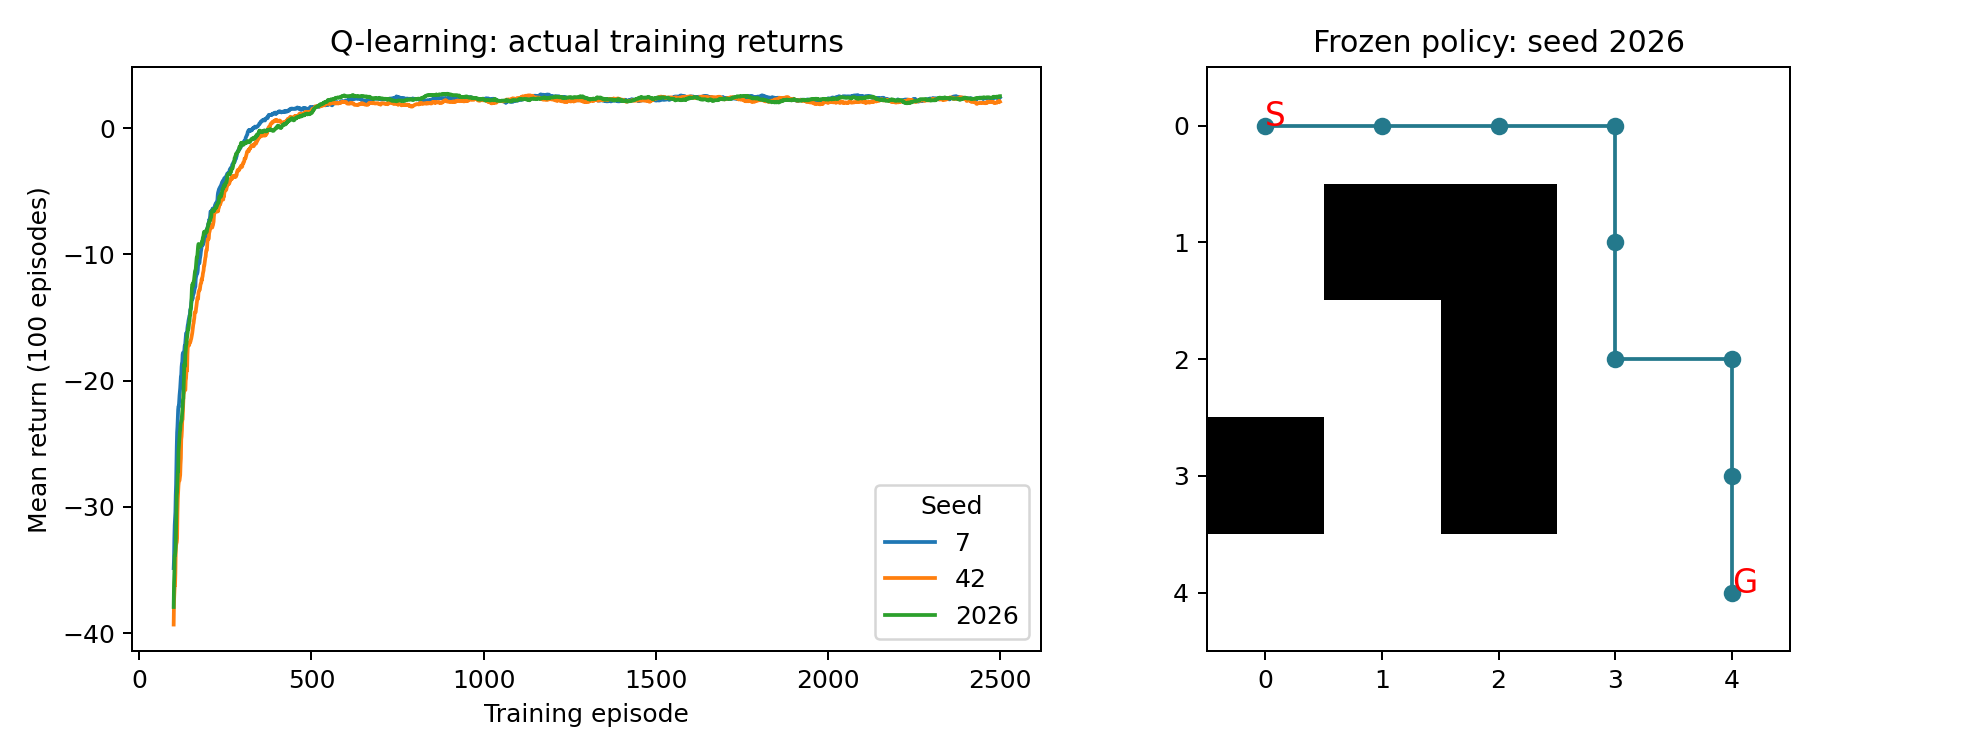
\includegraphics[width=\linewidth]{assets/q_learning_results.png}
\captionof{figure}{Kết quả Q-learning do code notebook sinh ra: reward huấn luyện và quỹ đạo đánh giá.}
\end{center}

\begin{center}\small
\begin{tabularx}{\linewidth}{@{}p{3.1cm}XXX@{}}\toprule
\textbf{Tiêu chí} & \textbf{Agent tìm kiếm} & \textbf{Trợ lý tra cứu} & \textbf{Agent Q-learning}\\\midrule
Quyết định & BFS trên mô hình & Chính sách Python cố định & Epsilon-greedy theo Q\\
Bộ nhớ & Cạnh bị chặn & Cache theo phiên bản & Bảng giá trị học được\\
Phản hồi & Di chuyển được/bị chặn & Hits, văn bản, lỗi schema & Trạng thái, reward, done\\
Thứ thay đổi & Kế hoạch và mô hình cục bộ & Kết quả cache & Giá trị Q qua episode\\
Bằng chứng & Nhật ký, 5 ca kiểm tra & 8 kiểm tra contract/nguồn & 3 seed, baseline, oracle\\
Giới hạn & Đồ thị nhỏ, cạnh không mở lại & Kho nhỏ, lexical, không LLM & Một lưới tĩnh, không chuyển miền\\\bottomrule
\end{tabularx}\end{center}

\subsection{Những gì ba bài thực hành chứng minh}
Bài 1 cho thấy phản hồi công cụ có thể làm thay đổi kế hoạch. Bài 2 cho thấy có thể
đặt giới hạn cho công cụ và gắn câu trả lời với tài liệu được đọc. Bài 3 cho thấy
một learning agent thực sự thay đổi bảng giá trị qua tương tác và được đánh giá
bằng chính sách đóng băng. Các chương trình dùng cơ chế khác nhau nên không được
gọi chung là LLM agent hoặc xem cập nhật cache là huấn luyện mô hình.

\subsection{Hướng mở rộng có thể thực hiện tiếp}
Để tiến gần ứng dụng thật, có thể thay dữ liệu giả lập bằng kho được cấp quyền,
thêm bộ chọn hành động dùng LLM với hợp đồng tool giữ nguyên, kiểm tra nguồn nhiều
đoạn và đánh giá trên tập câu hỏi độc lập. Với RL, có thể thêm bản đồ mới và nhiễu;
với tìm đường, có thể dùng trọng số cạnh và thời hạn bộ nhớ. Mỗi mở rộng cần báo
cáo lại dữ liệu, cấu hình, chi phí và tiêu chuẩn thành công.

\subsection{Kết luận chung của báo cáo}
Hiểu agent đầy đủ cần kết nối mục tiêu, biểu diễn trạng thái, lựa chọn hành động,
công cụ, phản hồi và kiểm chứng. Các tài liệu nghiên cứu mở rộng giúp phân biệt
những thành phần thường được ghép trong một ứng dụng hiện đại. Phần code hoàn chỉnh
và output đi kèm cho phép kiểm tra trực tiếp những kết luận thực nghiệm trong phạm
vi đã trình bày; các hướng đề xuất được tách khỏi phần đã chạy và đã đo.


\subsection{Nguồn dữ liệu và khả năng tái lập}
Các đường dẫn được chuẩn hóa về trang gốc, bỏ tham số theo dõi và chuyển hướng Facebook.
Các trang web có thể thay đổi nội dung theo thời gian; các URL được đối chiếu ngày
23/10/2026. Danh mục gồm 24 nguồn; các bài nghiên cứu được dẫn ở mục sử dụng tương ứng.
Nội dung tổng hợp được diễn đạt lại; các ví dụ đặt phòng,
xử lý phiếu và đồ thị thực nghiệm là phân tích, thiết kế riêng trong báo cáo, không
phải số liệu thực nghiệm của các tổ chức được trích dẫn.

Notebook đi kèm lưu đủ 17 cell code và output đã chạy. Tệp Python đi kèm xuất toàn bộ
code thực thi; ba bài không sử dụng API key hay lời gọi LLM giả lập.
Ảnh được chụp từ bản xuất HTML
của các cell bằng Chrome headless. Chạy lại bằng Jupyter với Python 3 và lựa chọn
\textit{Restart Kernel and Run All Cells}. Tệp \texttt{build\_notebook.py} cho phép dựng
lại notebook và HTML bằng IPython; các kiểm tra dùng \texttt{assert} nên lỗi kiểm tra
sẽ khiến quá trình dừng.
